% \begin{abstract}

% Tensor kernels in machine learning (ML)
%   often correspond to pure mathematical expressions,
%   making term rewriting an attractive strategy
%   for optimization and mapping to specialized hardware accelerators.
% %   ---%
% %   especially given recent progress in equality saturation.
% However,
%   existing ML intermediate representations (IRs)
%   tend to either be \textit{pure but high-level},
%   making low-level rewrites
%   to hardware targets inexpressible,
%   or \textit{low-level but impure},
%   hampering the use of term rewriting altogether.
% %   leaving no suitable IR
% %   for term rewriting
% %   over low-level tensor kernels.

% This paper introduces \g,
%   a pure IR whose core abstraction---%
%   the \textit{access pattern}---%
%   enables
%   low-level,
%   layout-aware,
%   hardware-centric
%   program rewrites.
% We demonstrate how term rewriting
%   in \g
%   can be used to 
%   map program fragments
%   to hardware accelerator invocations
%   and
%   automatically discover
%   classic data layout transformations
%   like \tcd{im2col}.
% % Hm... not capturing this idea at the moment:
% %  that facilitate hardware--software mapping
% %  but previously required explicit manual implementation.
% \g establishes a new foundation for
%   exploring further term rewriting techniques
%   in optimizing low-level tensor programs.
% %  \hl{todo we don't ever explain hardware--software programs}



% \end{abstract}

\chapter{Glenside}
\label{chapter:part1-glenside}

\textit{This chapter is derived from Smith et al.~\cite{smith2021pure}.}

\section{Introduction}

\hl{should this stuff be moved up to 3LA?}

Machine learning (ML) and other
  high-performance computing (HPC)
  applications increasingly rely on
  specialized hardware accelerators to
  provide speed and energy efficiency~\cite{jouppi2017tpu, krizhevsky2012conv, reuther2019survey}.
This trend has highlighted the need
  for flexible accelerator support
  in domain-specific compilers like
  Halide~\cite{halide},
  TVM~\cite{chen2018tvm},
  TensorFlow/MLIR~\cite{tensorflow, mlir}, and
  PyTorch~\cite{pytorch}.

Adding accelerator support to
  an existing compiler typically
  uses custom pattern matching to
  map expensive tensor operations
  from applications down to
  accelerator invocations~\cite{
    yang2020interstellar, byoc}.
Pattern matching often additionally relies on
  various other transformations
  to canonicalize intermediate representations (IRs)
  %~\cite{??}
  and massage data layouts into
  formats matching accelerator requirements~\cite{nvidia2020nhwc}.
Even with these changes,
  users may need to manually modify their application to
  help the compiler discover opportunities
  for dispatching operations to accelerators, 
  such as by changing data types or unrolling loops.
    
In principle, term rewriting techniques~\cite{baader1998term}
  should be able to facilitate many of
  these transformation and mapping tasks
  within a compiler.
Halide and TVM already rely
  on extensive rewrite systems for
  optimizing scalar computations and
  simplifying loop bounds in order to
  support further downstream optimizations~\cite{newcomb2020halide-rewrite,
  hagedorn2020func-high-perf}.

Unfortunately, existing IRs in compilers for
  array/tensor programming DSLs tend to
  present abstraction and granularity mismatches
  that hamper term rewriting approaches.
Term rewriting is most easily applied in
  \textit{pure} (side effect--free) IRs
  that support equational reasoning.
At the same time,
  mapping to accelerators requires considering
  low-level hardware details like data layout.
Existing pure IRs for ML frameworks are used
  primarily for high-level transformations
  (e.g., type elaboration and inlining)
  and do not expose low-level data layout details~\cite{relay}.
On the other hand,
  IRs used for crucial lower-level optimizations like
  operator fusion must support
  precise reasoning about memory use,
  and therefore are typically impure,
  hampering term rewriting.% approaches.

To help mitigate such impedance mismatches,
  we present \textit{\g},\footnote{Publicly available at \url{https://github.com/gussmith23/glenside}.}
  a pure tensor program IR
  that enables hardware-level term rewriting.
\g is based on a simple
  \textit{access pattern} abstraction that
  supports expressing and reasoning about
  data layout transformations via
  syntactic rewrite rules.
% We moved this figure elsewhere in the thesis
%   \begin{wrapfigure}{r}{.5\textwidth}
%     \centering
%     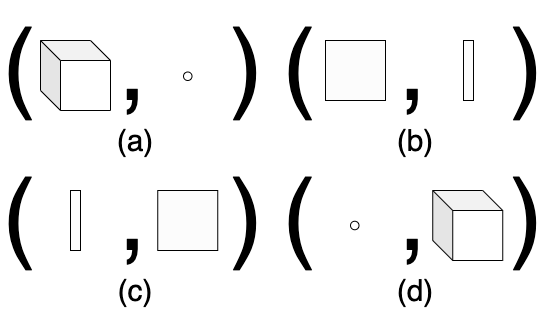
\includegraphics[width=.9\linewidth]{glenside/access-pattern-examples-2x2.png}
%     \caption{
%       Four access patterns,
%         representing different ways
%         a
%         tensor program
%         (or \textit{kernel})
%         might access
%         the same 3D tensor. 
%       For example, (c) represents
%         accessing a 3D tensor as
%         a vector of 2D matrices.}
%     \label{fig:access-pattern-examples}
%     \vspace{-1em}
% \end{wrapfigure}
When combined with standard arithmetic rewrites
  for per-tensor-element computations,
  access patterns enable implementing complex
  transformations for accelerator support as
  compositions of simple rewrites.

Tensors are traditionally characterized
  by their \textit{shape},
  an $n$-tuple 
  %in $\mathbb{N}^n$
  of positive integers
  indicating the size of each
  of a tensor's dimensions.
  % , e.g., $(x, y, z)$ for a 3D tensor.
Access patterns instead characterize
  each tensor with two shapes, e.g.,
  \accesspatternshape{x}{y, z}, separating
  the dimensions which are \textit{iterated over} from
  the dimensions which are \textit{computed on.}
Figure~\ref{fig:access-pattern-examples}(c)
  depicts an example where a 3D tensor's
  first dimension is iterated over and
  some computation applied to each
  corresponding 2D matrix.

We demonstrate how \g
  enables implementing representative
  hardware-level transformation via term rewriting,
  including mapping computations
  to systolic arrays~\cite{jouppi2017tpu}
  (a common hardware module in ML accelerators)
  and automatically discovering the
  \tcd{im2col} data layout transformation~\cite{im2col},
  which enables mapping 2D convolutions
  to matrix multiplication hardware.
In particular,
  by employing \textit{equality saturation}~\cite{willsey2021egg},
  these transformations ``fall out for free''
  (i.e., without any carefully crafted
  rewrite orderings~\cite{phase-ordering}),
  from a handful of general rewrites concerning tensor
  transposition, Cartesian product, dot product, etc.,
  expressed in terms of access patterns.

To summarize, the contributions of this chapter include:
\begin{itemize}
\item \textit{Access patterns},
  a tensor representation that employs a
  simple, extended tensor shape type to
  distinguish iteration and computation dimensions

\item The \g IR,
  a pure compiler IR that facilitates 
  term rewriting to enable support for
  specialized accelerators
  
\item A library of generic rewrites over \g programs
  
% \item Case studies demonstrating how
%   \g enables automatically discovering
%   key transformations for mapping
%   applications to custom accelerators
%   via equality saturation with the
%   \tcd{egg}~\cite{willsey2021egg} library.
\end{itemize}

\hl{i moved related work, so probably need to rework this}
The rest of this chapter is organized as follows:
Section~\hl{todo} provides background
  and briefly surveys closely related work.
Section~\hl{todo} motivates
  \g via a running example exploring
  pure matrix multiplication.
Section~\hl{todo} details the
  design and implementation of \g.


\section{From Pure \texttt{matMul} to IR Design Goals}
\label{sec:matmul}

% Many ML and HPC workloads are dominated by
%   evaluating compositions of tensor algebra operators
%   which, at a high level, correspond to
%   pure mathematical expressions.
% This make functional programming techniques attractive,
%   but requires careful design to ensure that
%   nested operators remain compositional with
%   respect to their output shapes.
% To highlight these design constraints and
%   motivate access patterns,
%   in this section we walk through a simple
%   matrix multiplication example to
%   illustrate the pitfalls that access patterns in \g
%   help mitigate.
  
Applying functional techniques
  and term rewriting to tensor IRs
  requires careful design.
For example,
  we must ensure that operators be compositional
  with respect to tensor shapes
  and that the representation support
  generic rules within the
  target rewrite engine.
To highlight such constraints and
  motivate access patterns in \g,
  this section illustrates potential pitfalls
  with a simple matrix multiplication example.

\subsection{Pure Matrix Multiplication}
\label{subsec:pure-matmul}

We write
  \tcd{f64} for the type of 64-bit floats and
  \tcd{[A]} for vectors over type \tcd{A}.
Using this notation, we can specify operators like
  dot product and 2D matrix transpose as:
\begin{align*}
    \mcd{dotProd} &
    \mcd{ : [f64] * [f64] -> f64} \\
    \mcd{trans2} &
    \mcd{ : [[f64]] -> [[f64]]}
\end{align*} 

% \begin{itemize}[leftmargin=*]
% \item
%   \tcd{[[f64]]} as the type of 2D matrices

% \item
%   \tcd{trans2 : [[f64]] -> [[f64]]} as matrix transpose

% \item 
%   \tcd{dotProd : [f64] * [f64] -> [f64]} 
%   as dot product
% \end{itemize}

%   so that, e.g.,
%   \tcd{[f64] * [f64] -> [f64]} represents
%   the type of a dot product operator \tcd{dotProd},
%   \tcd{[[f64]]} represents the type of
%   2D matrices of 64-bit floats, and
%   \tcd{[f64] * [f64] -> [f64]} represents
%   the type of a dot product operator.

% \noindent
% Assuming row-major layout,
%   implementing 2D matrix multiplication
%   on inputs \tcd{P} and \tcd{Q},
%   requires computing an output matrix
%   \tcd{R} such that:
% $$
%   \mcd{R[i][j] = dotProd(P[i],\, trans2(Q)[j])}
% $$

\noindent
Implementing 2D matrix multiplication
  on inputs $P$ and $Q$ requires computing
  an output matrix $R$ where
  $R_{ij} = \Sigma_k P_{ik} \, Q_{kj}
          =  P_i \cdot Q^{T}_{j}$. %\mcd{dotProd}(P_i, Q^{T}_{j}).$ 
The need to compute \tcd{dotProd} for every pair
  of a row from $P$ and a column from $Q$
  suggests map and Cartesian product operators
  which we might specify with:
\begin{align*}
    \mcd{map} &
    \mcd{ : (A -> B) * [A] -> [B]} \\
    \mcd{cartProd} &
    \mcd{ : [A] * [B] -> [A * B]}
\end{align*}
Naively, we can almost implement matrix multiplication as:
{\color{red} \begin{align*}
  & \mcd{matMul(P, Q) :=} \\
  & \;\;\;\;\; \mcd{map(dotProd, cartProd(P, trans2(Q)))}
\end{align*} }
% {\color{red} $$
%   \mcd{map(dotProd, cartProd(P, trans2(Q)))}
% $$ }
However, the result type will have been
  flattened to just {\color{red}\tcd{[f64]}},
  making it impossible to compose with other matrix
  operators that expect \tcd{[[f64]]} inputs.

Our first problem is that
  the \tcd{cartProd} specification above
  ``forgets'' the shape of its arguments.
We could change this specification to
  arrange the output as a matrix:
  % according to  the positions of its argument's indices
$$
  \mcd{cartProd2D : [A] * [B] -> [[A * B]]}
$$
But this result type prevents
  directly mapping \tcd{dotProd}.\footnote{
    This simple type does not specify how
    \tcd{cartProd2D} orders its output
    relative to its input vectors.
    We assume the order
    expected for matrix multiplication.}
Now the problem is that \tcd{map}
  only applies a computation by iterating
  over the first (outermost) dimension of a tensor.
If we specialize \tcd{map} to iterate
  over the second dimension:
$$
  \mcd{mapAt2 : (A -> B) * [[A]] -> [[B]]}
$$
then we can implement a compositional
  \tcd{matMul} operator that correctly produces
  results of type \tcd{[[f64]]} as:
\begin{align*}
  & \mcd{matMul(P, Q) :=} \\
  & \;\;\;\;\; \mcd{mapAt2(dotProd, cartProd2D(P, trans2(Q)))}
\end{align*}

While this gets us close
  to our goal of a pure, functional
  IR for tensor programs,
  as we'll see,
  this style also has its issues.

\subsection{\g Design Constraints and Goals}

This style of pure, higher-order functional
  program representation enables
  term rewriting and equational reasoning
  via rules like:
\begin{align*}
  \mcd{dotProd(P, Q)}
    & \leftrightsquigarrow
      \mcd{dotProd(Q, P)} \\[2pt]
  \mcd{trans2(trans2(P))}
    & \leftrightsquigarrow
      P \\[2pt]
  \mcd{map(f, map(g, P))}
    & \leftrightsquigarrow
      \mcd{map(f$\,\circ\,$g, P)} \\[2pt]
  \mcd{mapAt2(f, trans2(P))}
    & \leftrightsquigarrow
      \mcd{trans2(mapAt2(f, P))} % \\[2pt]
\end{align*}

% \footnote{
%     In these rules, we assume \tcd{reduce}
%     (``\tcd{fold}'') requires its first argument
%     to be an associative and commutative operator.}
%   \mcd{reduce(f, trans2(P))}
%     & \leftrightsquigarrow
%       \mcd{reduce(f, P)} \\[2pt]
%   \mcd{reduce(f, cartProd(P, Q))}
%     & \leftrightsquigarrow \\
%       \omit\rlap{\tcd{\hspace{0.5in}
%          reduce(f$\,\circ\,$swap, cartProd(Q, P))}}

However, some of these rules depend on the
  shapes of dimension-specific operators aligning.
What happens when we need to support
  higher-dimensional tensors?
Without a mechanism to abstract
  which dimensions of a tensor
  are being iterated as opposed to computed over,
  we would have to generate versions of
  each rule for every combination of dimensions.
Worse, these problems
  do not only affect rewrite rules;
  they also lead to code blowup just to
  specify all the variants of tensor kernels
  that arise in practice---%
  e.g.~we would eventually need
  \texttt{mapAt3}, \texttt{mapAt4},
  and so on.

One strategy to address these challenges is
  adding support for anonymous functions (``lambdas''),
  currying, and closures to the 
  tensor program representation.
These features can provide sufficient
  flexibility to handle shape alignment
  issues that otherwise may require
  dimension-specific operators like
  \tcd{cartProd2D} and \tcd{mapAt2} above.
For example, given curried versions
  of \tcd{dotProd} and \tcd{map},
  we could have used such features
  to implement a curried \tcd{matMul} as:
\begin{align*}
  & \mcd{matMul' P Q :=} \\
  & \;\; \mcd{ \
      map' ($\boldsymbol\lambda\,$r =>\
        map' (dotProd' r) (trans2 Q)) P}
\end{align*}
Alternatively, some IRs rely on index notation
  for even pithier implementations like:
$$
  \mcd{matMul(P,Q)[i,j] := dotProd(P[i], trans2(Q)[j])}
$$

Unfortunately, these approaches all rely on some
  form of \textit{name binding} which can
  significantly complicate term rewriting.
Rewriting under binders,
  whether explicitly in the form of lambdas
  or implicitly with index notation,
  requires additionally analyzing the
  potential \textit{contexts}
  (what names are bound to)
  of every subexpression.
While it is still technically possible to
  apply state-of-the-art rewrite engines
  like \tcd{egg}~\cite{willsey2021egg}
  via explicit variable substitution rules and
  free variable analyses,
  we have found the additional complexity
  and rewrite search space blow up
  substantially eliminate the potential advantages
  of term rewriting in such IR designs.

All the above constraints inform \g's key design goal:
  providing an IR that flexibly supports specifying and
  composing higher-order tensor operators\footnote{
    As \tcd{map} and \tcd{mapAt2} in 
    Section~\ref{subsec:pure-matmul} illustrate,
    an IR can support higher-order operators without
    necessarily providing lambdas, currying, or closures.}
  over arbitrary dimensions while still enabling
  high-performance term rewriting techniques
  like equality saturation.
In the rest of \cref{part:glenside-and-3la},
  we show how \textit{access patterns} enable achieving
  these goals with a focus on applications to
  mapping application fragments down to
  specialized hardware accelerators.

%\hl{
%Need to be explicit somewhere that access patterns,
%especially things like cartesian product,
%can just be for specification -- you 
%do not necessarily have
%to materialize everything.}

%\hl{(Probably worth saying that rewrite systems need pure IRs. Maybe consider a phrasing like this --Steve) ``However, rewrite systems are generally defined over pure languages---how will we represent matrix multiplication in a pure IR?''}
  
%{\color{red} \noindent\rule{8.5cm}{10pt}}


% {\color{red} \begin{align*}
%     & \mcd{matMul(A, B) :=} \\
%     & \;\;\;\; \mcd{map(dotProd, cartProd(A, trans2(B)))}
% \end{align*} }

% $$ 
% {\color{red}
%   \mcd{cartProd : [f64] * [f64] -> [f64 * f64]}
% }
% $$




% %To understand
% %  the genesis
% %  of access patterns,
% %  let's walk through
% %  an example.
% Let us consider an example
%   to motivate 
%   the access pattern representation.
% %Imagine 
% %  we'd like to build
% %  a simple term rewriting system
% %  to map matrix multiplications
% %  to an accelerator.
% %  we've built.
% Suppose we would like
%   to use 
%   a simple term rewriting system 
%   to map matrix multiplications
%   to an accelerator.
% Before we can start building rewrites,
%   we need to
%   represent our programs of interest---%
%   beginning with matrix multiplication---%
%   in a pure IR.

% Recall 
%   the matrix multiplication
%   algorithm:
%   given two two-dimensional tensors
%   $a$ and $b$
%   with shapes
%   $(M, N)$
%   and
%   $(N, O)$,
%   respectively,
%   we take the dot product
%   of every row of $a$
%   with every column of $b$,
%   to produce a new tensor
%   with shape $(M, O)$.
% The English description
%   of the algorithm
%   immediately suggests
%   a pure
%   representation,
%   shown in
%   Figure \ref{fig:matmul-haskell} left.
% Assume
%   \texttt{a}
%   and \texttt{b}
%   are two-dimensional tensors
%   with
%   some tensor type.
% Here,
%   we use a simple implementation
%   for our tensor type:
%   lists of lists,
%   \texttt{[[f64]]}.
% \texttt{(rows a)}
%   and \texttt{(cols b)}
%   produce lists
%   of the rows of \texttt{a}
%   and the columns of \texttt{b},
%   respectively.
% Using our nested-lists
%   tensor type,
%   \texttt{rows}
%   is simply
%   the identity function,
%   and \texttt{cols}
%   is a transpose function.
% \texttt{cartProd}
%   returns every element 
%   of the first list
%   paired with every element
%   of the second list;
%   in this case, 
%   every row of \texttt{a}
%   paired with
%   every column of \texttt{b}.
% \texttt{dotProduct}
%   computes the dot product
%   of two vectors.
% Putting it all together,
%   we \texttt{map}
%   the \texttt{dotProduct}
%   over our row--column pairs,
%   producing a result
%   with type
%   \texttt{[f64]}.
  
% Something doesn't seem right about this.
% The result
%   of multiplying
%   two two-dimensional tensors
%   should be a 
%   two-dimensional tensor,
%   not a one-dimensional list.
% Our program
%   computes the right values,
%   but it loses
%  a key piece of information:
%   the shape
%   of the resulting tensor.
% % I'm not actually sure we need to explain why shape is important.
% %Preserving
% %  shape information
% %  in a tensor-based
% %  program
% %  is essential.
% %Shape
% %  is the de facto way
% %  in which type
% %  information
% %  is conveyed
% %  in many tensor-based programs.
% %Perhaps
% %  the most common example
% %  is in activation layouts:
% %  an activation layout
% %  of \texttt{NCHW},
% %  for example,
% %  conveys which dimension
% %  is the batch dimension
% %  (\texttt{N}),
% %  which dimension is the channel
% %  dimension
% %  (\texttt{C}),
% %  and which dimensions
% %  are the spatial dimensions
% %  (\texttt{H} and
% %    \texttt{W}),
% %  and their order.
% Let's understand
%   where
%   the shape information
%   was lost.
% Both
%   \texttt{rows}
%   and
%   \texttt{cols}
%   preserve shape information,
%   which we can see
%   from their type,
%   \texttt{[[f64]] -> [[f64]]}.
% What about
%   \texttt{cartProd}?
% Its type signature
%   is
%   \texttt{[f64] -> [f64] -> [(f64, f64)]};
%   given two lists,
%   it returns a list of tuples.
% This new list
%   is of length
%   \texttt{length l0 * length l1}
%   for lists
%   \texttt{l0} and \texttt{l1}.
% In our example,
%   \texttt{rows a}
%   is a list of length $M$
%   of lists of length $N$,
%   and \texttt{cols b}
%   is a list of length $O$
%   of lists of length $N$.
% Thus,
%   \texttt{cartProd}
%   produces a list of length
%   $M \cdot O$
%   of 2-tuples
%   containing lists of length $N$.
% By the time
%   we map
%   \texttt{dotProduct}
%   over this list,
%   the shape information
%   has already been lost;
%   \texttt{dotProduct}
%   simply produces
%   another list
%   of length $M \cdot O$,
%   but with scalar values.
% It would seem
%   shape information
%   is lost
%   by \texttt{cartProd}.

% What
%   were we expecting
%   the result 
%   of \texttt{cartProd}
%   to be?
% We expect
%   the result of
%   the entire \texttt{map} expression
%   to be a tensor
%   with shape
%   $(M, O)$;
%   that is,
%   the outermost dimensions
%   of the original two inputs
%   ($M$ and $O$, respectively)
%   need to be preserved
%   \textit{separately,}
%   rather than
%   being \textit{flattened}
%   into a single dimension
%   of length $M \cdot O$.
% %Thus,
% %  the result of
% %  \texttt{cartProd}
% %  should presumably
% %  have a shape like
% %  $(M, O, \dots)$,
% %  rather than
% %  $(M*O, \dots)$.
% This brings us
%   to our first core obstacle:
%   we are using
%   the
%   one-dimensional list
%   semantics
%   of common functions
%   such as
%   \texttt{cartProd},
%   when
%   we need more complex semantics
%   for our more complex
%   tensor type.
  
% As a first pass
%   at this obstacle,
%   we can redefine
%   \texttt{cartProd}
%   to preserve
%   shape information.
% Its type signature
%   will change
%   from
%   \texttt{[f64] -> [f64] -> [(f64, f64)]}
%   to
%   \texttt{[f64] -> [f64] -> [[(f64, f64)]]}.
% That is,
%   rather than producing
%   a single list
%   whose length is a product
%   of the input lists' lengths,
%   we will produce a list of lists,
%   or a two-dimensional tensor.
% This
%   preserves
%   our shape information.
  
% Now, though,
%   we are presented
%   with another problem;
%   how should \texttt{map}
%   work
%   over our tensor representation?
% Currently,
%   \texttt{map}'s type
%   is 
%   \texttt{(f64 -> f64) -> [f64] -> [f64]};
%   thus,
%   it will attempt to map
%   our uncurried
%   \texttt{dotProduct}
%   over only 
%   the \textit{outermost}
%   dimension
%   of the result of 
%   \texttt{cartProd}.
% Not only
%   is this not what we want---%
%   it is also 
%   a type error.
% By preserving
%   the shape information
%   through
%   \texttt{cartProd},
%   we have necessitated
%   a more complex
%   implementation
%   of \texttt{map}.
% Specifically,
%   \texttt{map}
%   needs to understand
%   which dimensions
%   of the input tensor
%   should be considered the
%   ``list'' dimensions,
%   unaffected by the map,
%   and which dimensions
%   should be considered
%   the ``item'' dimensions,
%   which represent
%   the data structure
%   being passed in
%   to the function.
% In this case,
%   we want
%   \texttt{map}
%   to map the function
%   over the tuples
%   contained in the second
%   level
%   of lists.
% Figure \ref{fig:matmul-haskell} right
%   shows
%   our updated 
%   matrix multiplication,
%   using a new function,
%   \texttt{tensorMap2},
%   which treats
%   tensor dimensions
%   0 and 1
%   as ``list'' dimensions
%   and maps a function
%   over dimension 2
%   and above.

% With our change to
%   \texttt{cartProd}
%   and our new version
%   of \texttt{map},
%   we finally have
%   a functional representation
%   of matrix multiplication.
% Using this representation,
%   we can start writing rewrite rules
%   for our hardware accelerator,
%   in terms of
%   \tcd{tensorMap2},
%   \tcd{dotProduct}, and
%   \tcd{cartProd}.
% However,
%   these operators
%   are defined
%   for our specific
%   two-dimensional
%   usecase,
%   and thus, the rewrite would be brittle;
%   if $a$ or $b$
%   had more dimensions,
%   we would again
%   need to redefine
%   \texttt{map},
%   \texttt{cartProd},
%   and our rewrite as a whole.
  
% \texttt{cartProd}
%   and
%   \texttt{tensorMap2}
%   are conveying
%   which dimensions
%   of the input tensors
%   are being \textit{iterated over}
%   and which are
%   being \textit{computed on}.
% But instead
%   of conveying
%   this information
%   in these functions'
%   types,
%   it
%   could instead
%   be conveyed 
%   by the type
%   of the tensor itself.
% This is the core insight
%   of access patterns,
%   which we will now describe.
  
\section{\g}
\label{sec:glenside}
  
% Trying to get this to end up on the right page...
\begin{table*}
\small
    \centering
    \caption{\g's access pattern transformers.}
    \label{tab:access-pattern-transformers}
    \begin{tabularx}{\linewidth}{lXX}
    Transformer 
    & Input(s)
    & Output Shape  \\
    \hline
    
    %%%%%% ACCESS
    \texttt{access} 
    &
    \accesspatternshape{a_0,\dots}{\dots, a_n}
    and non-negative integer $i$
    & 
  \accesspatternshape
  {a_0, \dots, a_{i-1}}{a_i,\dots, a_n}
    \\
    
    %%%%% TRANSPOSE
    \texttt{transpose} &
    \accesspatternshape{a_0,\dots}{\dots, a_n},  $\ell$ (a permutation of $(0, \dots, n-1)$) &
    \accesspatternshape{a_{\ell_0},\dots}{\dots, a_{\ell_n}}
    \\
    
    \texttt{cartProd} 
    &
    \accesspatternshape{a_0,\dots, a_n}{c_0, \dots, c_p},  \accesspatternshape{b_0,\dots, b_m}{c_0, \dots, c_p}
    & 
  \accesspatternshape
  {a_0, \dots, a_n, b_0,\dots, b_m}
  {2, c_0, \dots, c_p}
    \\
    %...implementing the rows-by-columns data reading pattern used in matrix multiplication; implementing the filter--window pairing in \ctd{} \\
    
    %%%% WINDOWS
    \texttt{windows} 
    &
    \accesspatternshape{a_0, \dots, a_m}{b_0, \dots, b_n}, \newline
    window shape $(w_0, \dots, w_n)$,
    strides $(s_0, \dots, s_n)$
    &
    \accesspatternshape{a_0, \ldots, a_m, b'_0, \dots, b'_n}{w_0, \dots, w_n},\newline
    where $b'_i = \lceil (b_i - (k_i - 1)) / s_i \rceil $\\
    
    %%%% SLICE
    \texttt{slice} &
    \accesspatternshape{a_0, \dots }{\dots, a_n}, \newline
    dimension index $d$, bounds $[l, h)$
    &
    \accesspatternshape{a'_0, \dots }{\dots, a'_n} \newline
    with $a'_i = a_i$ except $a'_d = h - l$
    \\
    %...accessing a subset of a tensor \\
    
    \texttt{squeeze} &
    \accesspatternshape{a_0, \dots }{\dots, a_n}, index $d$ where $a_d = 1$
    &
    \accesspatternshape{a_0, \dots }{\dots, a_n} with $a_d$ removed
    \\
    
    \texttt{flatten} &
    \accesspatternshape{a_0,\dots,a_m}{b_0,\dots,b_n} &
    \accesspatternshape{a_0 \cdots a_m}{b_0 \cdots b_n} \\
    
    \texttt{reshape} &
    \accesspatternshape{a_0,\dots,a_m}{b_0,\dots,b_n},\newline
    access pattern shape literal
    \accesspatternshape{c_0,\dots,c_p}{d_0,\dots,d_q}&
    
    \accesspatternshape{c_0,\dots,c_p}{d_0,\dots,d_q},\newline
    if $a_0 \cdots a_m = c_0 \cdots c_p$
    and $b_0 \cdots b_n = d_0 \cdots d_q$\\
    
    %%% PAIR
    \texttt{pair}&
    two access patterns of shape
  \accesspatternshape
  {a_0, \dots}{\dots, a_n} &
  \accesspatternshape
  {a_0, \dots}{2, \dots, a_n}
    \\
    
    \end{tabularx}
\end{table*}

%\hl{Move up resolution of section 3 to beginning of section 4}

%\hl{max: do a bigger bomb drop. what have we done before we compute dot product? we've set up a complex system of accessing, which is completely separate from the computation that we're doing}

%\hl{the interesting thing is that these kernels end up looking very similar when you phrase them in glenside}

%\hl{need to say that we're solving the problem we set up}

%\hl{see, we've done what we said we're going to do}

This section details \g's implementation,
  focusing on its core abstraction,
  \textit{access patterns}.
We use Section~\ref{sec:matmul}'s
  matrix multiplication as a
  running example throughout.
  %beginning
  %with the definition
  %of access patterns,
  %then ways we can combine access patterns,
  %and finally,
  %describing how we compute over access %patterns.
%To illustrate,
   %we will progressively convert
   %the matrix multiplication example
   %from Section~\ref{sec:matmul}
   %to our final \g implementation.
  

\subsection{Access Patterns}

% Access patterns
%   encode a common trope
%   in tensor programs
%   in which
%   some of the dimensions of a tensor
%   are \textit{iterated over}/\textit{accessed}
%   while others are
%   \textit{computed on.}

Access patterns encode common
  tensor IR patterns where
  some tensor dimensions
  are \textit{iterated over} (accessed)
  while others are \textit{computed on}.\footnote{
    This is similar to NumPy's concept of \textit{universal functions.}}
Section~\ref{sec:matmul}'s \tcd{matMul} example
  \textit{iterates over} dimension 0 of input $P$,
  while \textit{computing on} dimension 1,
  effectively viewing $P$ as a 1D vector of 1D vectors.

Access patterns are specified by their \textit{shape} ---
  a pair of tuples of positive integers $(S_A, S_C)$.
An access pattern of shape $(S_A, S_C)$ is, in turn, a
  tensor $T$ whose shape is given by the
  concatenation of the access pattern shape tuples
  $S_A \,\mcd{++}\, S_C$; we refer to
  $S_A$ and $S_C$ as the \textit{access} and
  \textit{compute}
  dimensions of $T$, respectively.

Access patterns represent the view of an
  $(|S_A| + |S_C|)$--dimensional tensor
  as a tensor of shape $S_A$,
  each of whose elements has shape $S_C$.
For an access pattern $T$ of shape $(S_A, S_C)$
  where $|S_A| = n_A$, we use the syntax
  \tcd{(access $T$ $n_A$)} to represent $T$ in \g.
For example, if a 2D matrix $T$ has shape $(m, n)$,
  then the \g expression \tcd{(access $T$ 1)}
  yields an access pattern of shape $((m), (n))$.
  

% % We formally define access patterns
% %   as follows:
% An access pattern is defined by its
%   \textit{shape} ---
%   a pair of tuples
%   \accesspatternshape
%     {s_0, \dots, s_{m-1}}
%     {s_{m}, \dots, s_n}
%   where $s_i \in \mathbb{Z^+}$.
% An access pattern of shape
%   \accesspatternshape
%     {s_0, \dots, s_{m-1}}
%     {s_{m}, \dots, s_n}
%   is a tensor $t$
%   of shape
%   \[(s_0, \dots, s_{m-1},s_{m}, \dots, s_n)
%   \]
%   where $(s_0, \dots, s_{m-1})$
%   are called
%   its \textit{access} dimensions
%   and $(s_{m}, \dots, s_n)$
%   are called 
%   its \textit{compute} dimensions.
% The access pattern
%   represents the interpretation of $t$
%   as a tensor of shape
%   $(s_0, \dots, s_{m-1})$,
%   where every element
%   is a tensor
%   of shape
%   $(s_{m}, \dots, s_n)$.
% We call these
%   $(s_{m}, \dots, s_n)$-shaped
%   tensors
%   the access pattern's
%   \textit{subviews.}
% In \g,
%   we construct such an access  pattern
%   with the syntax
%   \texttt{(access t m)}.
% % With this definition,
% %   we now have the tools needed
% %   to represent
% %   our view of $P$
% %   in our matrix multiplication example.
% If a matrix $P$ has shape
%   $(M, N)$,
%   then the \g expression
%   \texttt{(access P 1)}
%   produces an access pattern
%   of shape
%   \accesspatternshape
%   {M}
%   {N}.
  
The matrix multiplication example
  from Section~\ref{sec:matmul}
  directly accesses the rows of $P$,
  but uses \tcd{trans2} to iterate over
  the columns of $Q$.
Instead of requiring an explicit
  transpose operator, \g provides
  access pattern \textit{transformers}.
  
\subsection{Access Pattern Transformers}

Access pattern transformers 
  manipulate one
  or more access patterns
  to produce a new access pattern,
  allowing \g
  to support more complex patterns
  like
  slicing,
  transposing,
  and interleaving.
  Table~\ref{tab:access-pattern-transformers}
  lists \g's transformers.
  
% So far in our matrix multiplication example,
%   we have created
%   an access pattern
%   \texttt{(access P 1)}
%   representing the rows of $P$.
To produce an access pattern
  representing
  the columns of $Q$
  for matrix multiplication,
  we employ
  the \texttt{transpose}
  transformer.
It takes an access pattern
  and a list of dimension indices,
  and rearranges
  the dimensions 
  of the access pattern
  in the order specified by the indices.
If $Q$ has shape $(N, O)$,
  \texttt{(transpose (access $Q$ 1) (list 1 0))}
  produces
  an access pattern
  of shape
  \accesspatternshape{O}{N}.
  
% Next,
%   matrix multiplication
%   requires
%   we implement
%   a Cartesian product.
% Section~\ref{sec:matmul} described the
%   challenges of representing
%   Cartesian products.
%   gave us trouble
%   under array-of-array
%   semantics
%   in \autoref{sec:matmul}.
% We were forced to define
%   \tcd{cartProd2D},
%   which was hard-coded
%   for our specific inputs
%   (2D tensors)
%   and our desired output
%   (pairs of the vectors in dimension 1
%     of the input tensors).
% However, access patterns
%   enable
%   a surprisingly intuitive 
%   and flexible definition.
The \texttt{cartProd} transformer
  takes access patterns
  of shapes
  \accesspatternshape{a_0, \dots, a_n}{c_0, \dots, c_p}
  and 
  \accesspatternshape{b_0, \dots, b_m}{c_0, \dots, c_p}
  respectively, and produces 
  an access pattern of the shape
  \accesspatternshape
    {a_0, \dots, a_n, b_0,\dots, b_m}
    {2, c_0, \dots, c_p},
  where $(2, c_0, \dots, c_p)$
  represents a 2-tuple
  of the input access patterns'
  compute dimensions.
The access dimensions
  of the input access patterns
  are simply concatenated.
In the matrix multiplication example,
  the Cartesian product
  of the rows of $P$
  with the columns of $Q$
  is an access pattern
  of shape
  \accesspatternshape{M,O}{2, N},
  where the second shape
  represents a 2-tuple
  of a row from $P$
  with a column from $Q$.

We have nearly re-implemented
  matrix multiplication example
  in \g.
The final step
  is to implement the dot product, for which
  \g uses 
  access pattern \textit{operators}.
  
\subsection{Access Pattern Operators}

\begin{table}
    \centering
    \caption{\g's access pattern operators.}
    \label{tab:operators}
    \begin{tabularx}{\linewidth}{lXX}
    Operator & Type & Description\\
    \hline
    \texttt{reduceSum} & $(\dots) \rightarrow ()$ &
    sum values
    \\
    
    \texttt{reduceMax} & $(\dots) \rightarrow ()$&
    max of all values\\
    
    \texttt{dotProd} &
    $(t,s_0, \dots, s_n)\rightarrow ()$ &
    eltwise mul; sum
    %eltwise.~mult.~$t$ tensors  of  shape $(s_0, \dots, s_n)$, reduce with  sum
    \\
    
% COPIED right from glenside source. just add to table as needed!
%        DotProduct,
%    ReduceSum,
%    ReLU,
%    Sqrt,
%    Negative,
%    /// Expects item shape of `a x b1 x .. x bn`. Performs an elementwise
%    /// addition of the `a` tensors of size `b1 x .. x bn`.
%    /// TODO(@gussmith) Multiple-arg compute feels clunky and ad-hoc.
%    /// Should figure out an explicit way to define access multiple-stream
%    /// access patterns.
%    ElementwiseAdd,
%    /// Expects item shape of `a x b1 x .. x bn`. Performs an elementwise
%    /// multiplication of the `a` tensors of size `b1 x .. x bn`.
%    ElementwiseMul,
%    ElementwiseDiv,
%    /// Takes the max across all elements in each item. Reduces any item shape
%    /// to a scalar.
%    ReduceMax,
%    /// Computes softmax. Currently expects access axis to be 0. Unsure how to
%    /// define softmax for other access patterns.
%    Softmax,
%    /// For an item shape of `a1 x a2 x ...`, returns an item shape of `1` where
%    /// the returned scalar is the mean of the `a1 x a2 x ...`-shaped tensor.
%    ReduceMean,

   
    \end{tabularx}
\end{table}

\textit{Operators}
  are the only \g
  constructs
  which
  perform computation.
They are invoked only
  in \texttt{compute} expressions,
  which map the operator
  over the compute dimensions
  of an access pattern.
For an input access pattern
  $A$
  of shape
  \accesspatternshape
  {s_0, \dots, s_{m-1}}
  {s_m, \dots, s_{n}},
  and an operator
  $f$
  with type
  $(s_m,\dots,s_n)
  \rightarrow
  (s'_{m'}, \dots, s'_{n'})$,
  the result of
  \texttt{(compute $f$ $A$)}
  will have shape
  \accesspatternshape
  {s_0, \dots, s_{m-1}}
  {s'_{m'}, \dots, s'_{n'}};
  that is, a \tcd{compute}
  expression
  cannot change
  the access dimensions
  of the input access pattern.
Table \ref{tab:operators}
  lists
  the operators
  in \g{}.
  
Recall where we are
  in converting
  our matrix multiplication
  example:
  we have accessed the rows of $P$
  and the columns of $Q$
  and taken their Cartesian product,
  resulting in an access pattern
  of shape
  \accesspatternshape
  {M, O}{2, N},
  and we need now
  to compute the dot product
  of these row-column
  pairs.
In \g,
  the \texttt{dotProd}
  operator
  (see Table~\ref{tab:operators})
  does just that.
To compute the dot product
  over our row-column pairs,
  we need only to apply
  \texttt{compute dotProd}
  to our access pattern,
  to produce an access pattern
  with final shape
  \accesspatternshape
  {M, N}{}.
The entire \g
  specification
  of matrix multiplication
  is shown in Figure \ref{fig:mat-mat-mult}.
  
\definecolor{gray}{Gray}{5} 
  
\begin{figure*}
\begin{minipage}{.54\textwidth}
\begin{subfigure}{\textwidth}
\begin{lstlisting}[basicstyle=\footnotesize,escapechar=!]
(transpose                   !\color{gray}; \hspace{2mm}\accesspatternshape{N, O, H', W'}{}!
 (squeeze                    !\color{gray}; \hspace{2mm}\accesspatternshape{N, H', W', O}{}!
  (compute dotProd           !\color{gray}; \hspace{2mm}\accesspatternshape{N, 1, H', W', O}{}!
   (cartProd                 !\color{gray}; \hspace{2mm}\accesspatternshape{N, 1, H', W', O}{2, C, K_h, K_w}!
    (windows                 !\color{gray}; \hspace{2mm}\accesspatternshape{N, 1, H', W'}{C, K_h, K_w}!
     (access activations 1)  !\color{gray}; \hspace{2mm}\accesspatternshape{N}{C,H,W}!
     (shape C Kh Kw)
     (shape 1 Sh Sw))
    (access weights 1)))     !\color{gray}; \hspace{2mm}\accesspatternshape{O}{C, K_h, K_w}!
  1)
 (list 0 3 1 2))
 
     \end{lstlisting}
       \vspace{-1.5em}
    \subcaption{2D convolution.
    %Activations in \texttt{NCHW} format; weights
    %in \texttt{OIHW} format.
    %\hl{do we describe NCHW/OIHW?}
    }
    \label{fig:conv2d}
\end{subfigure}
\end{minipage}
\begin{minipage}{.45\textwidth}

%%%%%% MATMUL
\begin{subfigure}{\textwidth}
\begin{lstlisting}[basicstyle=\footnotesize,escapechar=!]
(compute dotProd          !\color{gray}; \hspace{2mm}\accesspatternshape{M, O}{}!
 (cartProd                !\color{gray}; \hspace{2mm}\accesspatternshape{M, O}{2, N}!
  (access activations 1)  !\color{gray}; \hspace{2mm}\accesspatternshape{M}{N}!
  (transpose              !\color{gray}; \hspace{2mm}\accesspatternshape{O}{N}!
   (access weights 1)     !\color{gray}; \hspace{2mm}\accesspatternshape{N}{O}!
   (list 1 0))))
  \end{lstlisting}
  \vspace{-1.5em} 
  \subcaption{Matrix multiplication.}
  \label{fig:mat-mat-mult}
\end{subfigure}

%%%%% MAXPOOL
\begin{subfigure}{\textwidth}
\begin{lstlisting}[basicstyle=\footnotesize,escapechar=!]
(compute reduceMax       !\color{gray}; \accesspatternshape{N,C,H',W'}{}!
 (windows                !\color{gray}; \accesspatternshape{N,C,H',W'}{K_h, K_w}!
  (access activations 2) !\color{gray}; \accesspatternshape{N, C}{H, W}!
  (shape Kh Kw)
  (shape Sh Sw)))
\end{lstlisting}
  \vspace{-1em} 
  \subcaption{Max pooling.}
  \label{fig:maxpool-code}
\end{subfigure}

\end{minipage}
\caption{Common tensor kernels from machine learning expressed in \g. Lines containing access patterns are annotated with their access pattern shape.
$N$ is batch size; $H$/$W$ are spatial dimension sizes; $C$/$O$ are input/output channel count; $K_h$/$K_w$ are filter height/width; $S_h$/$S_w$ are strides.
}
\label{fig:all-kernels}
\end{figure*}

\section{\g in \TLA}
\label{sec:glenside-in-3la}

Now that we have presented
  \g,
  we will now briefly describe
  how \g was used within 3LA.

Operations which can be offloaded
  to accelerators
  can be captured via patterns,
  as discussed with 
  TVM's Bring Your Own Codegen
  framework.
Rather than attempt to enumerate all semantically equivalent patterns
 (a task that is tedious, error-prone, and likely to result in an incomplete enumeration), 
 or expect users to modify their application code to expose expected patterns (demanding knowledge of the model and patterns
  as well as engineering effort), 
  %, engineering time, and debugging effort),
   \TLA 
   increases the flexibility
   of compiler backend algorithms
  by utilizing term rewriting and \gls{equality-saturation} techniques to transform programs
  to expose the most  matching opportunities for accelerator operation selection. 
It is in this task
  that 
  \TLA uses \g.

Flexible matching uses two kinds of rewrite rules, both expressed in \g:
\begin{itemize}
\item Compiler IR rewrite rules: These are general-purpose \g-to-\g rules, independent of the accelerator, and are reusable and composable for various applications. We have developed a general set in \TLA %that is used across all our benchmarks. 
including rules for, e.g., merging/splitting tensors, commutativity, associativity, and identities for common operators. 
%\recheck{skip? These rules can also be extended by the system designer, e.g., in case of compiler IR updates, but in our experience they have largely stabilized and we expect they will be complete-in-practice for most users.}

\item \mapping rules: These rewrite rules are accelerator-specific,
  and translate from \g to black-box
  accelerator calls.
When targeting new accelerators, accelerator designers are expected to provide these mappings.
\end{itemize}

All rewrites in {\TLA} are polymorphic over tensor size, which requires specifying relationships between the input and output sizes for operations that merge, split, or broadcast over tensors. This also makes a given \mapping more general and provides support for applications using different block sizes, strides, etc., without changing any rules. 
%Note that this separation provides many benefits for compiler IR rewrites: (a) they become a one-time-cost that can be shared across accelerators, (b) one can use off-the-shelf term rewriting systems for implementing them, and (c) these rewrites can use purely functional IRs, without requiring bespoke compilation steps for state/effect analysis. 

In the extraction phase of equality saturation, the rewritten program optimizing the cost function is chosen. % as the final version of the program. 
This provides flexibility in the criteria for selection among functionally equivalent candidates for accelerator offloads. In our evaluations where we focused on end-to-end functional testing, we used a simple cost function that maximizes the number of accelerator invocations. More sophisticated cost functions can incorporate information about performance or data movement costs, and thereby result in different offloads.

%% Aarti: \iffalse around submitted text below
\iffalse
%\paragraph{Flexible Matching.} 
Specifically, we utilize equality saturation
  to perform ``\textit{flexible matching}'':
  The search applies \mapping rules %IR--ILA rewrites 
  to insert accelerator operations into the program,
  as well as equivalent rewrites within the compiler IR (compiler IR--compiler IR rewrites)
  to expose even more acceleration opportunities. % to apply accelerator operations.
  \iffalse
Equality saturation avoids
  phase-ordering issues when applying rewrites
  by searching over many equivalent rewritings of the same program,
  including different choices of accelerator operations,
  which ultimately reduces the need for manual program restructuring
  and improves application portability.
Given an input program $p$, 
  equality saturation repeatedly applies 
  the given rewrite rules 
  to explore all equivalent ways to express $p$
  (with respect to the rewrite rules).
This is accomplished using an \textit{e-graph} data structure
  to efficiently represent an exponentially large set of equivalent program expressions~\cite{nelson1980fast,nieuwenhuis2005proof}.
Upon reaching a fixed point, 
  i.e., when no application of any rewrite rule can introduce a new program expression, 
  the optimal rewritten program
  can be extracted from an e-graph
  according to a given cost function,
  thus providing for searching over many candidate rewritings without sophisticated ordering considerations.
\fi
%The use of equality saturation
  %also exposes opportunities for optimizations,
Since all rewritings with respect to the given rules 
  are available for the search,
  choosing an optimal rewriting
  reduces to framing the right cost function and search heuristics.
This allows %for automatically testing 
the use of \textit{unmodified} off-the-shelf applications
  and exploring all possible mappings to the accelerator operations (as demonstrated in our evaluation, \S\ref{sec.compilation-stats})---%
  a very useful capability during early design exploration. 
  
  %---requiring only a \textit{one-time} effort per accelerator
  %in the form of providing the compiler IR--accelerator rewrite rules.
%,
 % requires a \textit{one-time} effort per accelerator (the addition of compiler IR--accelerator rewrite rules),
  %and allows for exploring all possible mappings to the accelerator---%
  %a useful capability during early design exploration.
\fi 

\iffalse
Two additional advantages of our flexible-matching approach
  are that the general-purpose rewrite rules
  can be used with \emph{all} target accelerators and applications,
  %and thus require only a one-time effort to specify
  and that rewrite rules for multiple accelerators
  can be \emph{simultaneously} included, 
  %in the equality saturation,
  thereby searching over all opportunities 
  to invoke all available accelerators in concert.
In the extraction phase of equality saturation,
  the rewritten version maximizing the cost function
  is chosen as the final version of the program.
  This provides flexibility in the criteria for selection among functionally equivalent candidates for accelerator offloads.
  \fi 
%, by designing a suitable cost function.
%Because this approach often exposes more opportunities to invoke accelerators (\S\ref{sec.compilation-stats}), we refer to this approach as ``flexible matching,'' in contrast to ``exact.''
  %\aarti{add a forward pointer to flexible matching results}

\textit{Compiler IR rewrite rules.} Here, we describe three examples of compiler IR rewrite rules to show different types of opportunities that can be exposed.
%
\footnotesize
\begin{eqnarray} 
  \texttt{(compute dot-product (reshape \%x \%s))} &\rightarrow& \texttt{(reshape (compute dot-product \%x) \%s)} \label{rr-reshape-bubbling} \\
  \texttt{(add (reshape (dense \%a \%b) \%s) \%c)} &\rightarrow& \texttt{(reshape (bias\_add (dense \%a \%b) \%c) \%s)} \label{rr-linear-layer} \\
  \texttt{\%x} &\rightarrow& \texttt{(reshape (flatten \%x) (shape-of \%x))} \label{rr-flatten}
\end{eqnarray}
\normalsize
%
The \texttt{reshape} operator takes a tensor and a shape vector as input and re-arranges the layout of the tensor to the given shape, and the \texttt{dot-product} operator takes a tensor as input and computes the inner product of vectors under the given axis~\cite{smith2021pure}. Rule~\ref{rr-reshape-bubbling} exploits the properties of the two operators and shows that rearranging the application order of \texttt{reshape} and \texttt{dot-product} operators
  preserves the semantics.
Rule~\ref{rr-linear-layer} shows that linear layer \glspl{mlkernel} can be expressed 
  using different arrangement and combinations of operators, e.g., $\texttt{bias\_add}$ (broadcasting) or the 
  elementwise $\texttt{add}$.
Rule~\ref{rr-flatten} shows that de-simplifying a computation 
  (e.g., flattening then unflattening) could expose more opportunities for matching 
  rewrites.
Moreover, combining these individual rewrite rules together enables more 
  sophisticated rewrites. 
For example, combining Rule~\ref{rr-reshape-bubbling} and Rule~\ref{rr-flatten} 
  allows for the emerging $\texttt{im2col}$ transformations for convolution kernels, 
  without needing to specify the transformation as a new rewrite rule.

\iffalse
In addition to matching the compiler \mapping by adding them as rewrite rules 
  in Glenside, this approach also facilitates \emph{additional} matches through 
  the inclusion of \textit{general-purpose rewrite rules} within Glenside, such 
  as tensor shape transformations and algebraic manipulations of combinators.
  %including algebraic manipulations of various combinators in the language. 
%  \aarti{mention shape transformations here?}
These general-purpose rules
  allow the term-rewriting system to conclude
  that different variations of an expression
  (like the linear layer examples above)
  are, in fact, equivalent.
In our examples, using the rewrite rules in Glenside
  exposed acceleration opportunities in both
  the LSTM-WLM and ResNet-20 programs
  through specifying \textit{only a single}
  %compiler IR--ILA rewrite 
  \mapping rule for each accelerator operator.
  %we are able to annotate desirable accelerator operations in
  %both the LSTM-WLM and ResNet-20 implementations,
  %specifying only a single compiler IR--ILA rewrite for each accelerator operation
  %and relying on Glenside's general-purpose rewrite rules 
  %to expose opportunities to invoke the former.
% \todaes{[Mike] to rewrite this para and add explanation/examples of the rewrite rules.}

\todaes{Glenside IR and its rewrite rules support expressing commonly used deep learning kernels (e.g. nn\_dense, conv2d) as well as the underlying tensor-level computations. For example:
}
\begin{enumerate}
    \item \todaes{\textit{Equivalent linear layers using kernels}}
    \todaes{\[\texttt{(add (reshape (nn\_dense \%a \%b) \%s) \%c) => (reshape (bias\_add (nn\_dense \%a \%b) \%c) \%s)}\]
    % This  rule matches the pattern of a linear layer using elementwise addition and rewrites to an equivalent biased addition by pushing the \texttt{reshape} operator to the outer-most level.
}
    \item \todaes{\textit{Bubble reshape operators in tensor-level computations}}
    \todaes{\[\texttt{(compute dot-product (reshape \%x \%s)) => (reshape (compute dot-product \%x) \%s)}\]}
    \item \todaes{\textit{Flatten and unflatten tensors}}
    \todaes{\[\texttt{\%x => (reshape (flatten \%x) (shape-of \%x))}\]
    % This rewrite rule says that given an arbitrary tensor \texttt{\%x}, flattening \texttt{\%x} and reshaping it back to its original shape gives the same tensor. When combined with other rewrite rules (such as the one above), flexible matching in Glenside is able to perform \texttt{im2col} transformations for convolution kernels.
    }
\end{enumerate}
\todaes{The above rules embody three of the crucial properties of applications that make term-rewriting promising. Rule (1) shows that computations that can be rewritten into equivalent representations using different operations (such as using a $\texttt{bias\_add}$ instead of an elementwise $\texttt{add}$ by pushing out the $\texttt{reshape}$). Rule (2) exposes computations where rearranging the application of existing operations remains equivalent. Finally, rule (3) exemplifies how "de-simplifying" a computation can expose opportunities to offload. Exploring these properties together exposes more sophisticated offloads. For example, combining (3) with (2) allows the matching procedure to perform $\texttt{im2col}$ transformations for convolution kernels. These rewrite rules address the mismatch of static pattern matchers introduced in Sec \ref{sec.method.matching}.}
\fi

\textit{IR-to-accelerator mapping rules.}
Similar to compiler IR rewrite rules, we specify IR-to-accelerator mapping 
  rules in Glenside.
These rules are accelerator-specific, mapping supported 
  operations to accelerator invocations.
We now describe three examples of IR-to-accelerator mapping rules.
  %
\scriptsize
\begin{eqnarray}
  \texttt{(compute dot-product (cartesian-product ?x ?w))} &\rightarrow& \texttt{(vta-dense ?x ?w)} \label{rr-vta} \\
  \texttt{(conv2d ?input ?kernel ?group ...)} &\rightarrow& \texttt{(hlscnn-conv2d ?input ?kernel ?group)} \label{rr-hlscnn} \\
  \texttt{\{\{LSTM Relay Pattern\}\}} &\rightarrow& \texttt{(flexasr-lstm ?input ?hidden\_0 ...)} \label{rr-flexasr}
\end{eqnarray}
\normalsize
%
%The above rules showcase three ways to match and instantiate accelerator invocation operators: 
Rule~\ref{rr-vta} maps tensor-level computation of dense matrix multiplication 
  to VTA's \texttt{dense} operation. 
This allows matching decomposed coarse-grained operators and mapping to 
  fine-grained accelerator operations.
%Matching on tensor-level operations makes it easier to match computations decomposed from coarse-grained operators and map to accelerators with fine-grained computation supports. 
Rule~\ref{rr-hlscnn} maps kernel-level computation of a 2D convolution to 
  HLSCNN's \texttt{conv2d} operation---a common accelerator offloading for 
  deep learning kernels.
%This is a conventional way of using an accelerator to speed up computations of certain DL kernels. 
Rule~\ref{rr-flexasr} maps an LSTM computation to FlexASR's \texttt{lstm} operation.
Note that the LSTM computation (left-hand side) is specified using a pattern 
  compiled from a Relay program; this Glenside feature helps express complex
  operations.
%The left-hand side of Rule~\ref{rr-flexasr} denotes the LSTM computation pattern compiled from a Relay program that computes LSTM. This approach is useful when the computation is complicated and error-prone to write in \texttt{egg}. 
%Leveraging \texttt{egg}'s interface, these rewrite rules are all conditioned on predicates that check whether the corresponding accelerators support the set-up of the computation (e.g. dimensions of inputs, grouping of convolution kernels). 
%We omit the conditions here due to space constraints.

%\paragraph{Flexible matching via equality saturation}
%General-purpose rewrite rules and IR-to-accelertor mapping rewrite rules are implemented in Glenside~\cite{smith2021pure} using interfaces provided by \texttt{egg}~\cite{willsey2021egg}. 
%Leveraging equality saturation, these rules are applied exhaustively to input programs: general-purpose rewrite rules enable discovering semantically equivalent programs; IR-to-accelerator mapping rules match on all these equivalent programs and explore opportunities of offloading computations to corresponding accelerators.
\TLA utilizes equality saturation and the two types of rewrite rules to transform 
  programs, aiming to expose the most matching opportunities for accelerator 
  operation selection.
It was not clear \textit{a priori} whether flexible matching would be performant for accelerators with complex \mapping rules needed for available accelerator designs. Our evaluation results in the next chapter show that compiler IR rewrites can be combined effectively with a few \mapping rules in flexible matching, which finds more matches than exact matching in a reasonable time. 

